\documentclass[11pt, a4paper]{article}

\usepackage{amsmath}
\usepackage{amsfonts} %Matheschriften
\usepackage{amssymb} %Mathesymbole
%\usepackage{mathptmx} % Einstellung für Schriften und Sonderzeichen in mathematischen Umgebungen
                        % ändert SChriftfont
\usepackage{wasysym} % Stellt diverse Sonderzeichen bereit
\usepackage{siunitx}
\usepackage{float}
\usepackage{microtype}
\usepackage{graphicx}
\usepackage{hyperref}
\usepackage{xcolor}
\usepackage[section]{placeins}
% allows for temporary adjustment of side margins
\usepackage{changepage}
\usepackage{rotating}


\usepackage[ngerman]{babel}
\addto\captionsngerman{%
 \renewcommand{\abstractname}{Einleitung}}

\title{Versuch 1: Eigenschaften des Elektron}
\author{Team 2-13: Jascha Fricker, Benedict Brouwer}
\begin{document}
    \maketitle


    \tableofcontents

    \newpage

    \section{Einleitung}

    Bei diesem Versuch werden die Eigenschaften des Elektrons betrachtet und dazu zwei Experimente durchgeführt. Zunächst wird duch das Fadenstrahlrohr
    der Quotient $\frac{e}{m}$ (spezifische Elektronenladung) berechnet. Durch den Millikan-Versuch kann anschließend die Elementarladung $e$ bestimmt
    werden, sodass auch die Masse des Elektrons $m_e$ berechnet werden kann.

    \section{Bestimmung der spezifischen Elektronenladung}

    \subsection{Theorie}

    Im Fadenstrahlrohr werden die Elektronen durch ein elektrisches Feld beschleunigt. Die Endgeschwindigkeit kann durch gleichsetzten der Energien bestimmt werden.

    \begin{align}
    \frac{mv^2}{2} = E_{kin} &= E_{elek} = q \cdot U \label{geschw}\\
    \Rightarrow v &= \sqrt{\frac{2qU}{m}}
    \end{align}
    
    Das Magnetfeld $B$ der Helmholzspulen kann mithilfe der Biot-Savart-Gesetzes bestimmt werden.
    Mit dem Strom $I$, der Windungszahl $N$ und dem Radius $R$ ergibt sich für diesen Versuch:

    \begin{align}
        B = \frac{\mu_0 N I}{R} \cdot \frac{4}{5}^{\frac{3}{2}} \label{B-Helm}
    \end{align}

    Die spezifische Elektronenladung ist der Quotient aus Ladung und Masse $\frac{e}{m}$.
    Diese kann durch die Messung des Radius des Strahls im Fadenstrahlrohr bestimmt werden. Es gilt:

    \begin{align}
        \frac{mv^2}{r} = F_{rot} &= F_{mag} = q \cdot v \cdot B \\
        \overset{\text{(\ref{geschw})}}{\Rightarrow} \ \  \frac{q}{m} &= \frac{2U}{B^2 \cdot r^2} \label{qm_formel}
    \end{align}

    \subsection{Ergebnisse}
    \paragraph{Vorüberlegungen}

    Aus einer Beschleunigungsspannung von maximal $300 \si{V}$ kann die maximale Geschwindigkeit eines Elektrons mit Ladung $e$ im nichtrelativistischen Fall
    \begin{align}
        v = \sqrt{\frac{2 e U}{m_e}} = 1,02 \cdot 10^{7} \si{m/s} < 2,9 \cdot 10^{7} \si{m/s} = 10\% \cdot c
    \end{align}


    berechnet werden. Da diese kleiner als zehn Prozent der Lichtgeschwindigkeit ist, kann auch im weiteren nichtrelativistischen gerechnet werden
    Jetzt muss noch überprüft werden, ob die thermische Energie der Glühkathode die Messungen verfälschen könnte.
    \begin{align}
        v_{tmax} = \frac{v_{100V}}{100} = \frac{\sqrt{\frac{2 e \cdot 100 \si{V}}{m_e}}}{100} = 59310 \si{m \per s} \\
        E_{tmax} = \frac{m_e \cdot v_{tmax}^2}{2} = 1,602 \cdot 10^{-21} \si{J} = \frac{3}{2} k T_{max} \\
        \Rightarrow T_{max} = \frac{2 E_{tmax}}{3 k} = 77K
    \end{align}
    Die thermische Energie plus die Austrittsarbeit muss kleiner als $E_{tmax}$ sein, da sonst die Messungen verfälscht würden. Da die Austrittsarbeit des Material leider nicht bekannt ist, kann die eigenlich maximale Temperatur aber nicht bestimmt werden.


    \paragraph{Auswertung der Messungen}
        Zur Bestimmung des spezifischen Weiderstands wurden zwei Messreihen aufgenommen \a' 30 Durchführung jeweils mit konstantem B-Feld bzw. konstanter Beschleunigungsspannung mit unterschiedlichen Kreisradien. Dabei gibt es eineige Unsicherheiten zu beachten:
        \begin{table}[H]
            \centering
          

            \begin{tabular}{c | c}
                Messgröße & Unsicherheit \\ \hline
                Stromstärke der Helmholzspulen  & $2.5 \% \pm 0.1 \si{\ampere}$ \cite{vc130} \\
                Beschleunigungsspannung & $ 8\% \pm 8 \si{volt}$ \cite{vc120}\\
                Strichgenauhigkeit & $\pm 0.5 \si{mm}$ \\
                Ablesegenauhigkeit & $\pm 1 \si{mm}$\\
            \end{tabular}
        \end{table}
        
        Die Messdaten wurden durch den gewichteten Mittelwert \cite{ABW} mit dem zugehörigen internen bzw. externen Fehler für jeden Radius einzelnd gemittelt.
        Mit diesen Mittelwerten lässt sich unter berücksichtigung der Gaußschenfehlerfortpflanzung \cite{ABW} mittels Gleichung \ref{B-Helm} und \ref{qm_formel} die spezifische Elementarladung für jeden Radius berechen.
        \begin{table}[H]
            \centering

            \begin{tabular}{c | c | c | c}
                Radius &  $30 \si{mm}$ & $40 \si{mm}$& $50 \si{mm}$  \\ \hline
                Magnetfeld konstant & $1.96(44) * 10^{-11} \si{\coulomb\kilogram}$ & $1.76(39) * 10^{-11} \si{\coulomb\kilogram}$ &$1.74(38) * 10^{-11} \si{\coulomb\kilogram}$ \\
                Beschleunigungsspannung konstant& $1.81(30) * 10^{-11} \si{\coulomb\kilogram}$ & $1.79(29) * 10^{-11} \si{\coulomb\kilogram}$ &$1.84(30) * 10^{-11} \si{\coulomb\kilogram}$ \\

            \end{tabular}
        \end{table}
        






    \paragraph{Einfluss des Erdmagnetfeldes}
        Bei der Bestimmung spezifischen Elementarladung wurde zunächst der Effekt des Erdmagnetfeldes auf den Versuchsaufbau
        vernachlässigt. In Garching bertägt die magnetischen Feldstärke $B_{gar} = 48,7 \si{\micro\tesla}$ \cite[]{magnetic_field} bei einem Inklinationswinkel von $\Theta_{incl,gar} = 64.4\si{\degree}$ \cite[]{magnetic_field}. 
        Daraus folgt eine maximale senkrechete Komponente (in Bezug auf die Kreisbahnen) von 
        \begin{align}
        B_{\bot,gar} = B_{gar} \cdot \cos (\Theta_{incl,gar} = 21.0 \si{\micro\tesla})
        \end{align}
        Dies würde die von uns gemessenen spezifischen Elementarladung um ca. 0.03 \% beeinflussen was im Vergleich zu anderen
        Fehlerquellen vernachlässigbar ist. 
        Um diesen Effekt nachzuweisen bietet es sich an, den Versuchsaufbau so zu positionieren, dass das Erdmagnetfeld senkrecht zum Elektronenring steht.
        Anschließend wird der Versuchsaufbau um 180 \si{\degree} gedreht um den maximalen Effekt des Erdmagnetfeldes zu messen.
        Zur Abschätzung des Effekts lässt sich $B_{min,gar} = B - B_{gar}$ und $B_{max,gar} = B + B_{gar}$ mit einer Beispielspannung von $ U = 300 \si{\volt}$ in \ref{qm_formel} einsetzen.
        Daraus resultiert eine Differenz in den Radien von $5.5 \si{\milli\metre}$ welche  im messbaren Bereich liegt.

    

    \section{Millikan}

    In diesem Versuch werden Öltröpfchen mithilfe eines Elektischen Feldes mit und entgegen die Schwerkraft bewegt. Dadurch kann der Einfluss der E-Felds auf die Tröpfchen und der Radius der Tröpfchen und damit die Ladung dieser bestimmt werden.

    \subsection{Theorie}

    Durch vorraussetze eines Kräftegleichgewichts bei gleichförmiger Bewegung erhält man einen Radius
    \begin{align}
        r_0 = \frac{3}{2} \sqrt{\frac{\eta_{Luft} (v_{steig} + v_{sink})}{(\rho_{\ddot{Ol}} - \rho_{Luft}) \cdot g}}%{ \rho_{Öl} - \rho_{Luft} \cdot g }
    \end{align}
    Wobei $\rho$ die Dichte des jeweilligen Stoffes ist, $v_{steig}$ die Geschwindigkeit, mit der die Tröpfchen steigen und $v_{sink}$ die Geschwindigkeit, mit der die Tröpfchen sinken. Da die Tröpfchen so klein sind, muss die Viskosität mit einem Korrekturterm versehen werden:
    \begin{align}
        \nabla_{korr} = \nabla_{Luft}(1+\frac{A \lambda}{r_0})^{-1}
    \end{align}
    Hier wurden die Werte $A = 1,257$ und $\lambda = 72(2) \si{\nano\metre}$ eingesetzt.
    Auch der Tröpfchenradius muss korrigiert werden:
    \begin{align}
        r_{korr} = \sqrt{r_0^2 + \left(\frac{A \lambda}{2}\right)^2} - \left(\frac{A \lambda}{2}\right)
    \end{align}
    Damit kann dann die Ladung der Tröpfchen $q$ mit der Angelegten Spannung $U$ und dem Abstand der Platten $d$ bestimmt werden:
    \begin{align}
        q = \frac{3 \pi d}{U} \cdot \nabla_{korr} \cdot r_{korr} \cdot \left(v_{steig} - v_{sink}\right)
    \end{align}
    Wenn alles richtig berechnet wurde, müssten die Errechneten Werte vielfache der Elementarladung $e = 1.602 \cdot 10^{-19} \si{C}$ sein.

    \subsection{Ergebnisse}
    Um die Verteilung zu veranschaulichen, wurde im Graphen \ref{fig:milllikam} die Ladung $q$ gegen den errecchneten Radius $r_{korr}$ geplottet.
    \begin{figure}[h]
        \centering
        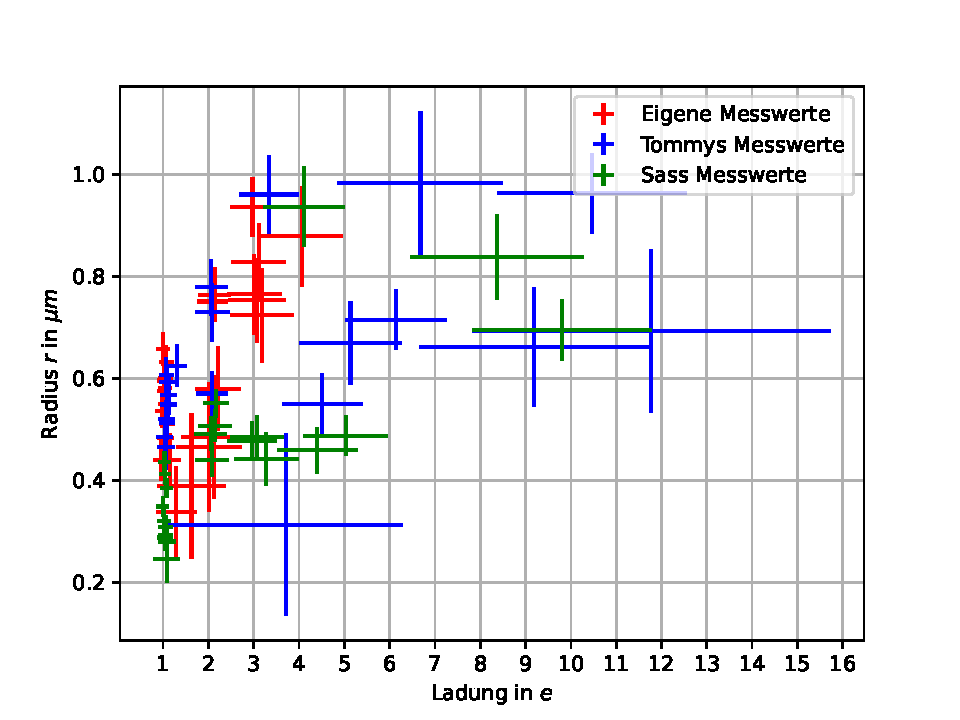
\includegraphics[width=0.8\textwidth]{millikan.pdf}
        \caption{Ladung der Tröpfchen und Radius im Milllikamversuch}
        \label{fig:milllikam}
    \end{figure}
    Außerdem wurde die Häufigkeitsvertielung der Ladungen im Graphen \ref{fig:hauf} ermittelt.
    
    Durch die Position der Maxima kann die Elementarladung bestimmt werden.

    Die in Tabele \ref{unsichmili} angegebenen Unisccherheiten wurden berücksichtigt.
    \begin{table}
        \begin{tabular}{c | c | c}
            Spannung $U$ in $\si{\volt}$ & 1 Digit = 1V & $u_U = \frac{1}{2\sqrt(3)} \si{\volt}$ \\
            Zeit $t$ in $\si{\second}$ & 1 Digit = 0,1s + Reaktionszeit 0,2s & $u_t = \sqrt(\frac{0.1}{2\sqrt(3)}^2 + 0.4) \si{\second}$ \\
            Abstand $s$ in $\si{\metre}$ & 1 Strich = 0,1mm & $u_s = \frac{0.0001}{4\sqrt(3)} \si{\metre}$ \\
            freie Weglänge $\lambda$ & Siehe \cite{ELE} & $u_\lambda = 2 \si{\nano\metre}$ \\
        \end{tabular}
        \caption{Unsicherheiten der Messwerte}
        \label{unsichmili}
    \end{table}
    Die Werte für Viskosität $\eta_{Luft}$ und Dichte $\rho_{Luft}$ der Luft \cite[]{Luft} sowie Dichte des Öls \cite{ELE} wurden ohne Unsicherheiten benutzt.




    \subsection{Diskussion}

    \bibliographystyle{plain}
    \bibliography{literature}

\end{document}